\documentclass[a4paper,12pt]{report}

\usepackage{fullpage}
\usepackage{url}
\usepackage{makeidx}
\usepackage{verbatim}
\usepackage{graphicx}
\input{./version.tex}

\newcommand{\caml}{\textsf{Caml}}
\newcommand{\pvs}{\textsf{PVS}\index{PVS@\textsf{PVS}}}
\newcommand{\coq}{\textsf{Coq}\index{Coq@\textsf{Coq}}}
\newcommand{\harvey}{\textsf{haRVey}\index{haRVey@\textsf{haRVey}}}
\newcommand{\simplify}{\textsf{Simplify}\index{Simplify@\textsf{Simplify}}}
\newcommand{\mizar}{\textsf{Mizar}\index{Mizar@\textsf{Mizar}}}
\newcommand{\hollight}{\textsf{HOL Light}\index{HOL Light@\textsf{HOL Light}}}
\newcommand{\isabelle}{\textsf{Isabelle/HOL}\index{Isabelle/HOL@\textsf{Isabelle/HOL}}}
\newcommand{\holfour}{\textsf{HOL 4}\index{HOL 4@\textsf{HOL 4}}}
\newcommand{\cvclite}{\textsf{CVC Lite}\index{CVC Lite@\textsf{CVC Lite}}}
\newcommand{\zenon}{\textsf{Zenon}\index{Zenon@\textsf{Zenon}}}
\newcommand{\krakatoa}{\textsf{Krakatoa}\index{Krakatoa@\textsf{Krakatoa}}}
\newcommand{\caduceus}{\textsf{Caduceus}\index{Caduceus@\textsf{Caduceus}}}
\newcommand{\java}{\textsc{Java}\index{Java@\textsf{Java}}}
\newcommand{\jml}{\textsc{JML}\index{JML@\textsf{JML}}}
\newcommand{\why}{\textsf{Why}}
\newcommand{\te}[1]{\texttt{#1}}
\newcommand{\nt}[1]{$\langle$\textsl{#1}$\rangle$}
\newcommand{\indexnt}[1]{\index{#1@\textsl{#1}, grammar entry}}
\newcommand{\indextt}[1]{\index{#1@\texttt{#1}}}
\newcommand{\etoile}{$^{\star}$}
\newcommand{\etoilesep}[1]{$^{\star}_#1$}
\newcommand{\plus}{$^+$}
\newcommand{\plussep}[1]{$^+_#1$}
\newcommand{\caveat}{\paragraph{Caveat.}}
\newcommand{\caveats}{\paragraph{Caveats.}}

\makeindex

\begin{document}

%%% coverpage
\thispagestyle{empty}
\begin{center}
~\\[3cm]
\rule\textwidth{0.1cm}\\[0.5cm]
{\Huge\sf The WHY verification tool}\\[1cm]
{\Large\sf Tutorial and Reference Manual}\\[0.1cm]
\rule\textwidth{0.1cm}\\[1cm]
Version \whyversion\\[3cm]
Jean-Christophe Filli\^atre
\vfill
\today\\
\end{center}


\tableofcontents

%%%%%%%%%%%%%%%%%%%%%%%%%%%%%%%%%%%%%%%%%%%%%%%%%%%%%%%%%%%%%%%%%%%%%%
\chapter*{Foreword}
\addcontentsline{toc}{chapter}{Foreword}

A computer program is telling the machine \emph{how} to compute some
output from its input. It is not giving the meaning of this
computation, nor the reason \emph{why} the program is correct. In the
best case, comments inserted in the code would give part of this
information. A formal method gives you the ability to tell the
machine both \emph{how} to compute and \emph{why} it is correct; hence
the name of this tool, \why.

% TODO

\medskip

This manual is organized as follows. Chapter~\ref{tutorial} gives an
overview of \why, illustrating all features with one-line examples.
Chapter~\ref{refman} is a reference manual.


\subsection*{License}

The \why\ certification tool is \copyright\ 2002--2006 Laboratoire de
Recherche en Informatique (\url{www.lri.fr}).
It is open source and freely available under the terms of the GNU
GENERAL PUBLIC LICENSE Version 2. See the files \texttt{COPYING} and
\texttt{GPL} in the distribution.


\subsection*{Availability}

The \why\ tool is available from \url{http://why.lri.fr/}, in source
and binary formats, together with this documentation and many
examples.


\subsection*{Contact}

There is a mailing list for \why, which is mainly used to announce the
releases. To subscribe, you need to send an email to
\url{why-request@serveur-listes.lri.fr} with 
\verb+subscribe your@email+ in the mail body. Emails can be sent to
the list at 
\url{why@serveur-listes.lri.fr}. Note: Only the lists members
can send emails to the list.

Bug reports can be sent to \url{filliatr@lri.fr}.



%%%%%%%%%%%%%%%%%%%%%%%%%%%%%%%%%%%%%%%%%%%%%%%%%%%%%%%%%%%%%%%%%%%%%%
\chapter{Quick tutorial}
\label{tutorial}

\section{Principles}

Basically, the \why\ tool takes annotated programs written in a very
simple imperative programming language of its own, produces verification
conditions and sends them to existing provers (proof assistants such
as Coq, PVS, etc. or automatic provers such as Simplify, CVC Lite,
etc.), as illustrated below:

\begin{center}
  \begin{tabular}{c}
    annotated programs \\
    $\downarrow$ \\
    \why \\
    $\downarrow$ \\
    verification conditions = first-order formulae \\
    $\downarrow$ \\
    \why \\
    $\downarrow$ \\
    external provers
  \end{tabular}
\end{center}

Simplify speaking, \why\ may be seen as an implementation
of Dijkstra's weakeast preconditions. Its key advantages are the
following: 
\begin{itemize}
\item 
  It is a verification condition generator (VCG) for a language
  specifically designed for the interpretation of existing programming
  languages. It includes the usual constructs of imperative
  programming and logical annotations (pre- and postconditions, loop
  invariants and variants, intermediate assertions) but also
  exceptions, recursive functions and polymorphism.

\item 
  The \why\ tool allows the declaration of logical \emph{models}
  (types, functions, predicates and axioms) that can be used in
  programs and annotations. Thus it is a highly generic VCG.  If one
  wants to model some kind of bounded precision arithmetic, for
  instance, it is as simple as declaring a new type and the
  corresponding operations (which may be defined later on the prover
  side, or left axiomatized).

\item
  The \why\ tool supports a wide set of existing provers
  (see Figure~\ref{fig:provers}). Thus verification conditions can be
  discharged by several provers independently. One may for instance
  use an interactive proof assistant to focus only on VC that are not
  automatically discharged by some (or any) automatic prover.
  Actually, the \why\ tool can be simply used as a front-end to all
  these provers, independently of its VCG mechanism. Then it is
  nothing more than a common first-order logic ``syntax'' for these
  provers. 

\end{itemize}

\begin{figure}
  \begin{center}
  \begin{tabular}{|l|l|l|}
    \hline
                     & Prover    & Command-line option 
    \\\hline\hline
    Proof assistants & Coq       & \texttt{-{}-coq}       \\\cline{2-3}
                     & PVS       & \texttt{-{}-pvs}       \\\cline{2-3}
                  & Isabelle/HOL & \texttt{-{}-isabelle}  \\\cline{2-3}
                     & HOL 4     & \texttt{-{}-hol4}      \\\cline{2-3}
                     & Hol Light & \texttt{-{}-hol-light} \\\cline{2-3}
                     & Mizar     & \texttt{-{}-mizar} 
    \\\hline\hline
    Automatic theorem provers 
                     & Simplify & \texttt{-{}-simplify} \\\cline{2-3}
                     & CVC Lite & \texttt{-{}-cvcl}     \\\cline{2-3}
                     & haRVey   & \texttt{-{}-harvey}   \\\cline{2-3}
                     & Zenon    & \texttt{-{}-zenon}    \\\cline{2-3}
                     & SMTlib   & \texttt{-{}-smtlib} 
    \\\hline
  \end{tabular}
  \end{center}
  \caption{Supported provers}
  \label{fig:provers}
\end{figure}


\section{A trivial example}

Here is a small example of \why\ input code:
\begin{verbatim}
  logic min: int, int -> int
  parameter r: int ref
  let f (n:int) = r := min !r n { r <= r@ }
\end{verbatim}
This code declares a function symbol \texttt{min} and gives its
arity. Whatever the status of this function is on the prover side
(primitive, user-defined, axiomatized, etc.), it simply needs to be
declared in order to be used in the following of the code. The next
line declares a parameter, that is a value that is not defined but
simply \emph{assumed} to exist i.e. to belong to the environment. Here
the parameter has name \texttt{r} and is an integer reference (\why's
concrete syntax is very close to Ocaml's syntax). The third line
defines a function \texttt{f} taking a integer \texttt{n} as argument
(the type has to be given since there is no type inference in \why)
and assigning to \texttt{r} the value of \texttt{min !r n}.
The function \texttt{f} has no precondition and a postcondition
expressing that the final value of \texttt{r} is smaller than its
initial value. The current value of a reference \texttt{x} is directly
denoted by \texttt{x} within annotations (not \texttt{!x}) and within
postconditions \texttt{x@} is the notation for the value of \texttt{x}
in the prestate (i.e. at the precondition point).

Let us assume the three lines code above to be in file
\texttt{test.why}. Then we can produce the proof obligations for this
program, to be verified with \coq, using the following command line:
\begin{verbatim}
  why --coq test.why
\end{verbatim}
A \coq\ file \texttt{test\_why.v} is produced which contains the
statement of a single proof obligation, which looks like
\begin{verbatim}
  Lemma f_po_1 : 
    forall (n: Z),
    forall (r: Z),
    forall (r0: Z),
    forall (HW_1: r0 = (min r n)),
    r0 <= r.
  Proof.
  (* FILL PROOF HERE *)
  Save.
\end{verbatim}
The proof itself has to be filled in by the user. If the \why\ input
code is modified and \why\ run again, only the statement of the proof
obligation will be updated and the remaining of the file (including
the proof) will be left unmodified.
Assuming that \texttt{min} is adequately defined in \coq, the proof
above is trivial.

Trying an automatic decision procedure instead of \coq\ is as easy as
running \why\ with a different command line option. For instance, to
use Simplify~\cite{Simplify}, we type in
\begin{verbatim}
  why --simplify test.why
\end{verbatim}
A Simplify input file \texttt{test\_why.sx} is produced. But Simplify
is not able to discharge the proof obligation, since the meaning of
\texttt{min} is unknown for Simplify:
\begin{verbatim}
  Simplify test_why.sx
  ...
  1: Invalid
\end{verbatim}
The user can edit the header of \texttt{test\_why.sx} to insert an
axiom for \texttt{min}. Alternatively, this axiom can be inserted
directly in the \why\ input code:
\begin{verbatim}
  logic min: int, int -> int
  axiom min_ax: forall x,y:int. min(x,y) <= x
  parameter r: int ref
  let f (n:int) = {} r := min !r n { r <= r@ }
\end{verbatim}
This way this axiom will be replicated in any prover selected by the
user. When using \coq, it is even possible to prove this axiom, though
it is not mandatory. With the addition of this axiom,
Simplify is now able to discharge the proof obligation:
\begin{verbatim}
  why --simplify test.why
  Simplify test_why.sx
  1: Valid.
\end{verbatim}

\section{A less trivial example: Dijkstra's Dutch flag}

Dijkstra's Dutch flag is a classical algorithm which sorts an array
where elements can have only three different values. Assuming that
these values are the three colors blue, white and red, the algorithm
restores the Dutch (or French :-) national flag within the array.
This algorithm can be coded with a few lines of C, as follows:
\begin{verbatim}
typedef enum { BLUE, WHITE, RED } color;

void swap(int t[], int i, int j) { color c = t[i]; t[i] = t[j]; t[j] = c;}

void flag(int t[], int n) {
  int b = 0, i = 0, r = n;
  while (i < r) {
    switch (t[i]) {
    case BLUE: swap(t, b++, i++); break;        
    case WHITE: i++; break;
    case RED: swap(t, --r, i); break;
    }
  }
}
\end{verbatim}

\indextt{type}\indextt{logic}\indextt{axiom}

We are going to show how to verify this algorithm---the
\emph{algorithm}, not the C code---using \why. 
First we introduce an abstract type \texttt{color} for the colors
together with three values \texttt{blue}, \texttt{white} and \texttt{red}:
\begin{verbatim}
  type color

  logic blue : color
  logic white : color
  logic red : color
\end{verbatim}
Such a new type is necessarily an \emph{immutable} datatype. The only
mutable values in \why\ are references (and they only contain
immutable values).

Then we introduce another type \texttt{color\_array} for
purely applicative arrays containing colors: 
\begin{verbatim}
  type color_array

  logic acc : color_array, int -> color
  logic upd : color_array, int, color -> color_array
\end{verbatim}
To get the usual theory of applicative arrays, we can add the
necessary axioms: 
\begin{verbatim}
  axiom acc_upd_eq : 
    forall t:color_array. forall i:int. forall c:color.
      acc(upd(t,i,c),i) = c
  axiom acc_upd_neq : 
    forall t:color_array. forall i:int. forall j:int. forall c:color.
      j<>i -> acc(upd(t,i,c),j) = acc(t,j)
\end{verbatim}

The program arrays will be references containing values of type
\texttt{color\_array}. In order to constraint accesses and updates to
be performed within arrays bounds, we add a notion of array length and
two ``programs'' \texttt{get} and \texttt{set} with adequate preconditions:
\begin{verbatim}
  logic length : color_array -> int

  axiom length_upd : 
    forall t:color_array. forall i:int. forall c:color.  
    length(upd(t,i,v)) = length(t)

  parameter get : 
    t:color_array ref -> i:int -> 
      { 0<=i<length(t) } color reads t { result=acc(t,i) }

  parameter set : 
    t:color_array ref -> i:int -> c:color -> 
      { 0<=i<length(t) } unit writes t { t=upd(t@,i,c) }
\end{verbatim}
These two programs need not being defined (they are only here to
insert assertions automatically), so we declare them as
parameters. 
As illustrated above, a function type has named arguments, a pre- and
a postcondition, a result type and an explicit declaration of its
side-effects: the \texttt{reads} and \texttt{writes} keywords
respectively declare the set of references possibly
accessed and modified.

We are now in position to define the \texttt{swap} function:
\begin{verbatim}
  let swap (t:color_array ref) (i:int) (j:int) =
    { 0 <= i < length(t) and 0 <= j < length(t) }
    let c = get t i in
    set t i (get t j);
    set t j c
    { t = upd(upd(t@,i,acc(t@,j)), j, acc(t@,i)) }
\end{verbatim}
The precondition for \texttt{swap} states that the two indices
\texttt{i} and \texttt{j} must lie within the array bounds and
the postcondition is simply a rephrasing of the code on the model
level i.e. on purely applicative arrays. Verifying the \texttt{swap}
function is immediate.

Next we need to give the main function a specification. First, we need
to express that the array only contains one of the three values
\texttt{blue}, \texttt{white} and \texttt{red}. Indeed, nothing
prevents the type \texttt{color} to be inhabitated with other values
(there is no notion of inductive type in \why\ logic, since it is
intended to be a common fragment of many tools, including many with no
primitive notion of inductive types). So we define the following predicate
\texttt{is\_color}:
\begin{verbatim}
  predicate is_color(c:color) = c=blue or c=white or c=red
\end{verbatim}
Note that this predicate is given a \emph{definition} in \why. 

Second, we need to express the main function postcondition that is,
for the final contents of the array,
the property of being ``sorted'' but also the property of being a
permutation of the initial contents of the array (a property usually
neglected but clearly as important as the former). For this purpose,
we introduce a predicate \texttt{monochrome} expressing that a set of 
successive elements is monochrome:
\begin{verbatim}
  predicate monochrome(t:color_array, i:int, j:int, c:color) =
    forall k:int. i<=k<j -> acc(t,k)=c
\end{verbatim}
For the permutation property, we simply \emph{declare} a predicate
\texttt{permutation}:
\begin{verbatim}
  logic permutation : color_array, color_array, int, int -> prop
\end{verbatim}
The intended meaning of \texttt{permutation($t_1$,$t_2$,$l$,$r$)} is
``the (multi-)sets of the elements of the sub-arrays $t_1[l..r]$ and
$t_2[l..r]$ are the same''. 

To be able to write down the code, we still need to translate the
\texttt{switch} statement into successive tests, and for this purpose
we need to be able to decide equality of the type \texttt{color}.
We can declare this ability with the following parameter:
\begin{verbatim}
  parameter eq_color  : 
    c1:color -> c2:color -> {} bool { if result then c1=c2 else c1<>c2 }
\end{verbatim}
Note that the meaning of \texttt{=} within annotations has nothing to
do with a boolean function deciding equality that we could use in
our programs.

We can now write the \why\ code for the main function:
\begin{verbatim}
let dutch_flag (t:color_array ref) (n:int) = 
  { length(t) = n and forall k:int. 0 <= k < n -> is_color(acc(t,k)) }
  let b = ref 0 in
  let i = ref 0 in
  let r = ref n in
  while !i < !r do
     if (eq_color (get t !i) blue) then begin
       swap t !b !i;
       b := !b + 1;
       i := !i + 1
     end else if (eq_color (get t !i) white) then
       i := !i + 1
     else begin
       r := !r - 1;
       swap t !r !i
     end
  done
  { (exists b:int. exists r:int. 
       monochrome(t,0,b,blue) and 
       monochrome(t,b,r,white) and 
       monochrome(t,r,n,red)) 
    and permutation(t,t@,0,n-1) }
\end{verbatim}
As given above, the code cannot be proved correct, since a loop
invariant is missing, and so is a termination argument. The loop
invariant must maintain the current situation, which can be depicted as
\begin{center}
  \begin{tabular}{|l|l|l|l|l}
    \multicolumn{1}{l}{0} & 
    \multicolumn{1}{l}{\texttt{b}} & 
    \multicolumn{1}{l}{\texttt{i}} & 
    \multicolumn{1}{l}{\texttt{r}} & 
    \multicolumn{1}{l}{\texttt{n}} \\\cline{1-4}
    \quad\texttt{BLUE}\quad~ & 
    \quad\texttt{WHITE}\quad~ & 
    \dots to do\dots & 
    \quad\texttt{RED}\quad~ \\\cline{1-4}
  \end{tabular}
\end{center}
But the loop invariant must also maintain less obvious properties such
as the invariance of the array length (which is obvious since we only performs
\texttt{upd} operations over the array, but we need not to loose this
property) and the permutation w.r.t. the initial array.
The termination is trivially ensured since \texttt{r-i} decreases at
each loop step and is bound by 0.
Finally, the loop is annotated as follows: 
\index{Loop invariant}%
\begin{verbatim}
  ...
  init:
  while !i < !r do
     { invariant 0 <= b <= i and i <= r <= n and
                 monochrome(t,0,b,blue) and 
                 monochrome(t,b,i,white) and 
                 monochrome(t,r,n,red) and
                 length(t) = n and
                 (forall k:int. 0 <= k < n -> is_color(acc(t,k))) and
                 permutation(t,t@init,0,n-1)
       variant r - i }
  ...
\end{verbatim}
A label \texttt{init} has been introduced right before the loop in
order to relate the current value of the array inside the loop
(denoted \texttt{t}) to its value right before the loop (denoted as
\texttt{t@init}) in the loop invariant.

To be able to perform the proof, we need to ``define'' the
\texttt{permutation} predicate.  The simplest way to do is to
axiomatize it as an equivalence relation containing the transpositions
within $[l..r]$:
\begin{verbatim}
  axiom permut_refl : forall t: color_array. forall l,r:int.
    permutation(t,t,l,r)

  axiom permut_swap : forall t:color_array. forall l,r,i,j:int.
    l <= i <= r -> l <= j <= r ->
    permutation(t, upd(upd(t,i,acc(t,j)), j, acc(t,i)), l, r)

  axiom permut_sym : forall t1,t2:color_array. forall l,r:int.
    permutation(t1,t2,l,r) -> permutation(t2,t1,l,r)

  axiom permut_trans : forall t1,t2,t3: color_array. forall l,r:int.
    permutation(t1,t2,l,r) -> permutation(t2,t3,l,r) -> 
    permutation(t1,t3,l,r)
\end{verbatim}
We have no way to state that this is the \emph{smallest} such relation
(this is not a first-order property) but this is not needed to show
the correctness of the program. Note: the loop invariant part related
to \texttt{is\_color} seems redundant since we should be able to
deduce it from the permutation property. But it would also require
induction, and thus it is simpler to add this property to the loop invariant.

We can now proceed to the verification of the program with
Simplify. We first produce the verification conditions in Simplify
syntax: 
\begin{verbatim}
  why --simplify flag.why
\end{verbatim}
Then we run Simplify on these obligations, using the tool \texttt{dp}
(distributed with \why; see~\ref{tool:dp}) that displays the results
of the automatic decision procedures in a nice way:
\begin{verbatim}
  dp flag_why.sx

(. = valid * = invalid # = timeout ! = failure)
flag_ax_why.sx: .......... (10/0/0)
total           :  10
valid           :  10 (100%)
invalid         :   0 (  0%)
timeout/failure :   0 (  0%)
\end{verbatim}
As we see, the 10 verification conditions are discharged by Simplify.
The source code of this example is part of the \why\ distribution, in
\texttt{examples/misc/flag\_ax.mlw}. 

\paragraph{Variants.} We describe here two variations around the Dutch
flag example.
\begin{itemize}
\item\textbf{Definition vs. axiomatization:} \indextt{external}
  Instead of axiomatizing some logical elements (such as
  the type \texttt{color} or the predicate \texttt{permutation} above), we
  can alternatively \emph{define} them on the prover side and simply
  \emph{declare} them in the \why\ source file. If we are using the
  \coq\ proof assistant, for instance, we could prefer defining the
  \texttt{color} type as an inductive data type, as follows:
\begin{verbatim}
  Inductive color : Set := blue : color | white : color | red : color.
\end{verbatim}
  Then we can declare these external elements in the \why\ source file
  as follows:
\begin{verbatim}
  external type color
  external logic blue, white, red : color
\end{verbatim}
  The \texttt{external} modifier indicates that nothing must be
  produced in the prover file for these declarations. Then we do not
  the \texttt{is\_color} property anymore, since we are able to prove
  (once on the \coq\ side) that there is no other value in the
  \texttt{color} type than \texttt{blue}, \texttt{white} and \texttt{red}.

  Similarly, we could define the \texttt{permutation} predicate as a
  \coq\ inductive predicate, and declare it in the \why\ source file
  as follows:
\begin{verbatim}
  external logic permutation : 
    color_array, color_array, int, int -> prop
\end{verbatim}

\item\textbf{Primitive arrays:} \index{Arrays}
  The \why\ tool actually provides a datatype of
  arrays, exactly in the way we have done it above i.e. an array is a
  reference on a purely applicative array.
  There is even a nice syntax for array operations:
  $t[e]$ stands for $(\mathtt{array\_get}~t~e)$
  and $t[e_1]:=e_2$ stands for $(\mathtt{array\_set}~t~e_1~e_2)$.
  This is part of the \why\ prelude, which is described on
  page~\pageref{prelude}. 

\end{itemize}

\section{Other features}

This section quickly describes additional features that were not
present in the example above.

\subsection{Assertions}\index{Assertion}\indextt{assert}
Assertions to be verified can be placed at any place inside code using the
\texttt{assert} construct. Example:
\begin{verbatim}
  begin 
    x := 2 * !x;
    assert { even(x) };
    x := !x - 1
  end
\end{verbatim}
An assertion can also be placed right \texttt{after} some program
expression using the postcondition construct:
\begin{verbatim}
  let x = (fib 4) { even(result) } in x+x
\end{verbatim}

Such assertions (before an expression with \texttt{assert} and after
with the brackets notation) can be used to introduce \emph{proof
  cuts}: first, they result in proof obligations at the corresponding
program point and then they are available in the context of the
following verification conditions. They are \emph{transparent}
i.e. they do not modify the information already available in the other
verification conditions.

There is also an \emph{opaque} variant of the postcondition construct,
which is written with double brackets:
\begin{verbatim}
  let x = (fib 4) {{ even(result) }} in x+x
\end{verbatim}
In that case, we still need to prove the property
\texttt{even(fib(4))} but, in the remaining of the program, we do not
know that \texttt{x=fib(4)} anymore. Only the property
\texttt{even(x)} is available.

\subsection{Recursive functions}
\index{Recursive function}
Recursive functions are introduced with the \texttt{let rec}
construct. They are annotated with a result type (there is no type
inference) and a variant to ensure termination.
For instance, the famous Mac Carthy's 91 function can be written as follows:
\begin{verbatim}
  let rec f91 (n:int) : int { variant max(0,101-n) } =
    if n <= 100 then
      (f91 (f91 (n + 11)))
    else
      n - 10
    { (n <= 100 and result = 91) or (n >= 101 and result = n - 10) }
\end{verbatim}

\subsection{Exceptions}
\index{Exception}\indextt{exception}\indextt{raises}

New exceptions are declared with the \texttt{exception} declaration and
may have arguments:
\begin{verbatim}
  exception E
  exception F of int
\end{verbatim}
Exceptions are raised with the construct \texttt{raise}:
\begin{verbatim}
     raise E
     raise (F 1)
\end{verbatim}
and caught with the construct \texttt{try \dots\ with \dots\ end}:
\begin{verbatim}
     try f 0 with E -> 1 end 
     try f 0 with F x -> x end
\end{verbatim}
It is not possible to catch an exception which is not possibly raised
by the expression following the \texttt{try}.

Postconditions are extended to specify the behavior in case of
uncaught exceptions:
\begin{verbatim}
     raise E { false | E => true }
     raise (F 1) { false | F => result = 1 }
\end{verbatim}
In a postcondition regarding an exception, \texttt{result} refers to
the value carried by the exception (if any).
In postconditions, it is not possible to mention exceptions which
are not possibly raised by the program.

In a function type, the exceptions possibly raised by the function
must be given as part of its side-effects, using the \texttt{raises}
keyword. For instance
\begin{verbatim}
  parameter f : x:int -> {} int raises E { P(x,result) | E => Q(x) }
\end{verbatim}
declares a function \texttt{f} taking an integer \texttt{x} as
argument, returning an integer and possibly raising the exception
\texttt{E}. In the latter case, \texttt{Q(x)} holds.

\subsection{Unreachable code}
\label{absurd}\indextt{absurd}

The \texttt{absurd} construct can be used to denote an unreachable
point in the code. Example:
\begin{verbatim}
     { 0 <= x <= 1 }
     if x = 0 then 
       ...
     else if x = 1 then 
       ...
     else 
       absurd
     { ... }
\end{verbatim}
At such program points, the user will be asked to prove that the
context is indeed absurd, which corresponds to the proof obligation
\texttt{false}. 

\subsection{Non-deterministic programs}
\index{Non-deterministic expression}

A non-deterministic program expression is a place-holder for a program
expression that is not given but only specified. Such a construct is
a program specification (a type, an effect and possibly some
pre/postconditions) written between square brackets. For instance
\begin{verbatim}
  [ {} int { even(result) } ]
\end{verbatim}
stands for any program expression of type \texttt{int} that has the
property of being even. Thus we can prove correct the following code:
\begin{verbatim}
  (1 + [ {} int { even(result) } ]) { odd(result) }
\end{verbatim}
This construct can be used to proceed by successive \emph{refinements}
or to write incomplete programs where only the meaningful parts are
coded. With respect to verification, a non-deterministic program
expression behaves like a call to a function parameter.

\section{Tools}\label{tools}

\subsection{Graphical user interface (\texttt{gwhy})}
\indextt{gwhy}\index{GUI}

The graphical user interface \texttt{gwhy} is a tool to help the user
in the process of calling the various automatic provers on the goals
(in order to analyze the failures and to determine what is wrong in
the programs, the specifications, or sometimes the provers).
\texttt{gwhy} is similar to \why\
and is passed the same options and files. A screenshort is given
Figure~\ref{fig:gwhy}. On the left side appears the list of all goals
(either from \texttt{goal} commands in the \why\ files or resulting
from verification conditions generation). In front of each goal, the
results for each automatic prover is displayed. Provers can be
launched by clicking on their names at the top of their columns.
A green bullet means a proved goal; a red bullet means an unproved
goal (that may be either a ``don't know'' or an ``invalid'' answer
from the prover); the scissors means a timeout from the prover (the
timeout limit can be set in the bottom bar); finally, a ``tools'' icon
means an unexpected failure in the prover call.

The top right window displays the currently selected goal.
In this window, a right click on some identifier displays its location
in the corresponding \why\ input file in the bottom right window.

\begin{figure}
  \centering
  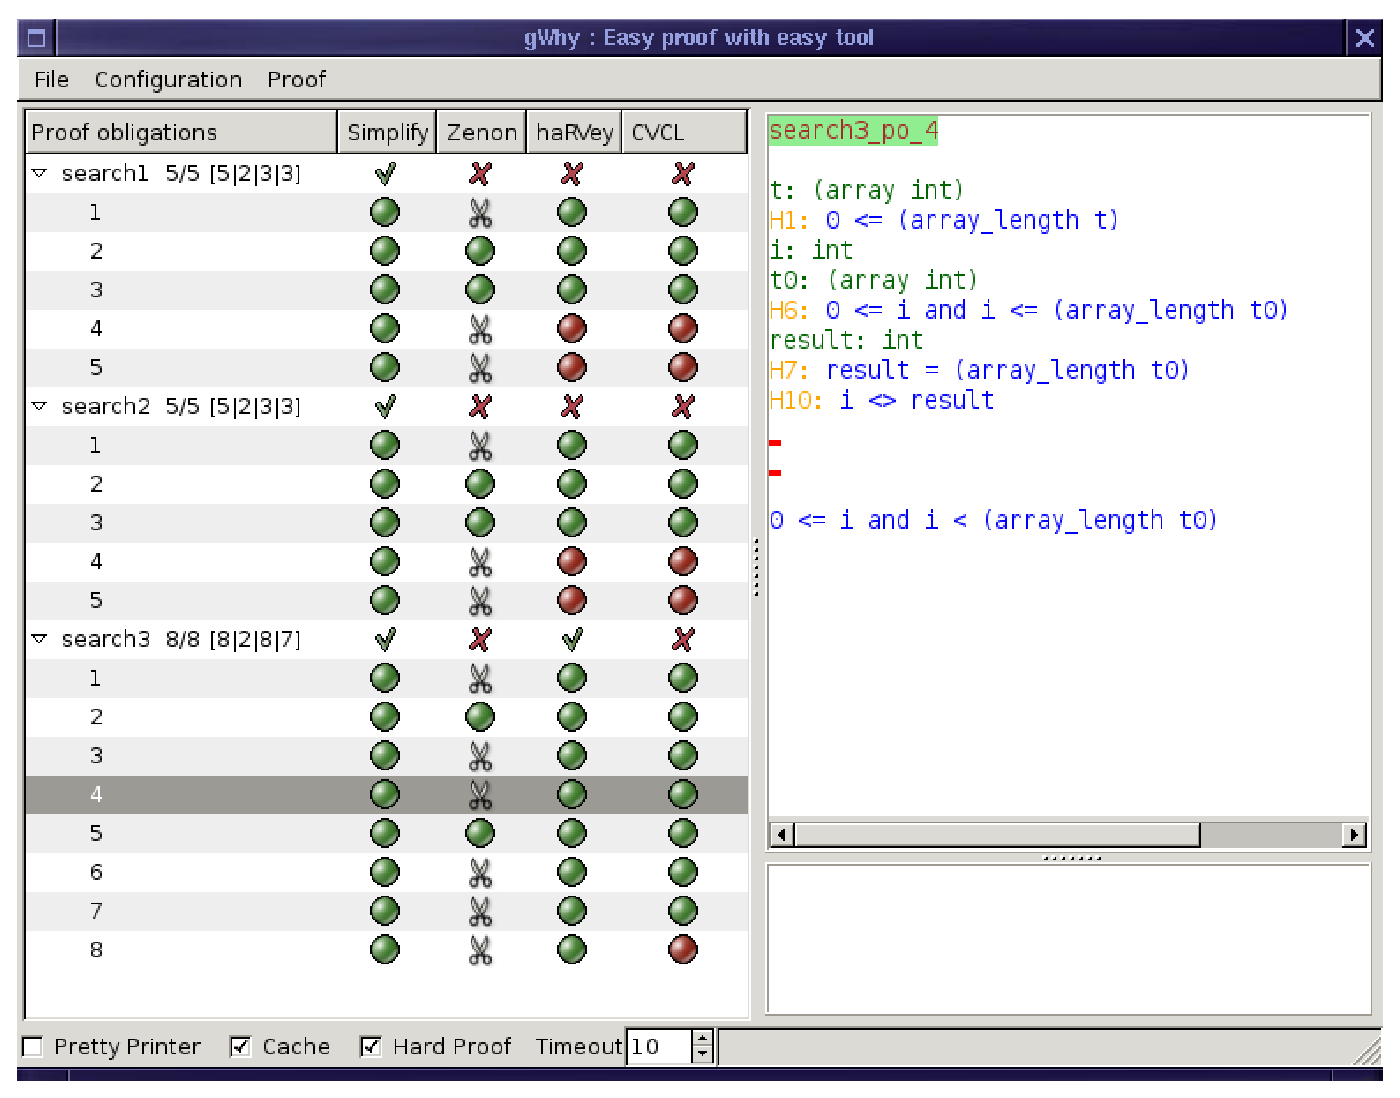
\includegraphics[width=0.8\textwidth]{gwhy-screenshot.eps}
  \caption{The \texttt{gwhy} graphical interface}
  \label{fig:gwhy}
\end{figure}

Note that you need the Unix \texttt{timeout} command to be installed
on your system before running \texttt{gwhy}.

\subsection{Calling decision procedures (\texttt{dp})}
\label{tool:dp}\indextt{dp}

A small tool is provided to call the decision procedures (\simplify,
\harvey, \zenon\ and \cvclite) on files containing several goals, with
a timeout for each goal, and to display s short summary of the
results. Here is an example:
\begin{verbatim}
% dp -timeout 5 swap0_why.sx peano_why.sx
(. = valid * = invalid # = timeout/failure)
swap0_why.sx: ....... (7/0/0)
peano_why.sx: ............*...*..*.... (21/3/0)
total           :  31
valid           :  28 ( 90%)
invalid         :   3 ( 10%)
timeout/failure :   0 (  0%)
\end{verbatim}

Note: as for \texttt{gwhy}, you need the Unix \texttt{timeout} command
to be installed on your system to run \texttt{dp}.

\subsection{Why obfuscator (\texttt{why-obfuscator})}
\indextt{why-obfuscator}
A tool is provided to obfuscate some \why\ files. It is invoked as
follows:
\begin{center}
  \texttt{why-obfuscator} [\texttt{-o}
  \textit{file}]�~�[\texttt{-prefix} \textit{p}]
  files...
\end{center}
It produces a \why\ file equivalent to the set of \why\ files given as
arguments, where all identifiers are renamed and all comments
removed. The output is printed on the standard output unless
redirected with option \texttt{-o}. The identifiers are renamed as
\texttt{x1}, \texttt{x2}, ... unless a different name prefix is set
with option \texttt{-prefix}.

\subsection{Why statistics (\texttt{why-stat})}
\indextt{why-stat}
A tool is provided to display rough statistics on the goals contained
in \why\ files. It is invoked as follows:
\begin{center}
  \texttt{why-stat} files...
\end{center}
It collects the symbols appearing in the conclusion of 
\texttt{goal} declarations, sums the number of goals with the same set
of symbols and displays this multi-set starting with the most numerous
elements. Here is a sample output:
\begin{verbatim}
       8 acc,shift
       2 valid
       1 valid_range
\end{verbatim}

\subsection{Caml code generation (\texttt{why --ocaml})}
\label{ocamlcode}\index{Caml code generation}
In order to run your \why\ code, true \caml\ code can be
produced with option \texttt{--ocaml}: 
\begin{verbatim}
     why --ocaml foo.mlw
\end{verbatim}
When this option is selected, there is no generation of proof
obligations (\coq\ or \pvs\ files are not produced or updated).
The \caml\ code is written on standard output, unless redirected to
some file with option \texttt{--output} (see Section~\ref{usage}).

Programs' annotations can be inserted as comments in the \caml\ code,
with option \texttt{--ocaml-annot}. The default behavior is no
annotation. 

When the input file contains \texttt{parameter} declarations, the
\caml\ code generated is a functor, with these parameters as
arguments. For instance, the following input file
\begin{verbatim}
     parameter x : int ref
     let f (y:int) = x := !x + y
\end{verbatim}
is translated into the following piece of \caml\ code:
\begin{verbatim}
     module type Parameters = sig
       val x : int ref
     end

     module Make(P : Parameters) = struct
       open P
       let f = fun y (*:int*) -> x := !x + y
     end
\end{verbatim}
\texttt{external parameter} declarations are supposed to be realized by some
external \caml\ code. However, it is possible to make them arguments
of the functor too, with command line option \texttt{--ocaml-ext}.

\subsection{Why to HTML converter (\texttt{why2html})}
\indextt{why2html}
A tool to convert \why\ input files to HTML is provided. Its usage is
immediate:
\begin{verbatim}
     why2html [-t title] files...
\end{verbatim}
Each \why\ input file given on the command line, say \textit{foo.mlw},
is translated into a HTML file \textit{foo.mlw.html}. A title for the
HTML page can be specified using command line option \texttt{-t};
otherwise the original file name is used.

\subsection{Simplify to Why converter (\texttt{simplify2why})}
\indextt{simplify2why}
A tool to convert Simplify files to Why syntax is provided. 
Its usage is immediate:
\begin{verbatim}
     simplify2why files...
\end{verbatim}
Each Simplify input file given on the command line, say \textit{foo.sx},
is translated into a \why\ file \textit{foo.sx.why}. Since Simplify is
untyped, all data in the Simplify input file are mapped to integers in
the resulting \why\ file.

\section{Installation}
\label{install}\index{Installation}

To compile \why, you need \textsf{Objective Caml} to be
installed, in version at least 3.08. It can 
be fetched from \url{http://caml.inria.fr}.
Then 

\begin{enumerate}
\item Configure with \texttt{./configure}

  The directory for binaries defaults to \texttt{/usr/local/bin}; you
  can specify another directory with the \texttt{-{}-bindir}
  option. Similarly, you can change the directory for the library
  with \texttt{-{}-libdir} and for
  the man pages \texttt{-{}-mandir}.

\item Compile with \texttt{make}.

\item Install with \texttt{make install}.
\end{enumerate}


\section{Examples}
\label{examples}\index{Examples}

Many examples are delivered with \why\ in the
subdirectory \texttt{examples/} of the distribution.
They are also available on the \why\ web site, at
\url{http://why.lri.fr/examples/}.


\section{Verifying C and Java programs}
\label{CandJava}

C and \java\ programs can be verified using other tools in combination
with \why. C programs can be verified using \caduceus\ (see
\url{caduceus.lri.fr/}) and \java\ programs using \krakatoa\ (see
\url{krakatoa.lri.fr}). 


\chapter{Reference manual}
\label{refman}


\section{Command line}
\label{usage}\index{Option, of the command line}

\why\ is invoked as a batch compiler, given a list of input files:
\begin{center}
  \texttt{why} [\textit{options}] \textit{file}$_1$ $\cdots$ \textit{file}$_n$
\end{center}
If no file is given, then standard input is processed and output is
named with the prefix \texttt{out\_why} (and a suffix depending of the
selected prover).
The full list of command line options can be obtained with
\begin{verbatim}
  why --help
\end{verbatim}



\section{Syntax of input files}
\label{syntax}

\subsection{Lexical conventions}

Comments are opened with \texttt{(*}, closed
with \texttt{*)} and can be nested.

Identifiers are made of letters, digits,
the underscore character \texttt{\_} and the single quote \texttt{'},
starting with a letter. Additionally, they can be qualified by a
label (another identifier), using the \texttt{@} notation.

\begin{center}
\begin{tabular}{lrl}
  \nt{identifier}\indexnt{identifier}
    & $::=$ & \nt{letter} (\nt{letter} $|$ \te{0}..\te{9} $|$
              \te{\_} $|$ \te{'})\etoile
  \\[0.1em]
  \nt{letter}
    & $::=$ & \te{A}..\te{Z} $|$ \te{a}..\te{z}
  \\[0.1em]
  \nt{lab\_identifier}\indexnt{lab\_identifier}
    & $::=$ & \nt{identifier} [ \te{@} [ \nt{identifier} ] ]
\end{tabular}
\end{center}

Keywords are the following:
\begin{center}
{\tt\begin{tabular}{l@{\qquad}l@{\qquad}l@{\qquad}l@{\qquad}l}
        absurd &
	and &
        array &
	as &
	assert \\
	axiom &
	begin &
        bool &
	do &
	done \\
        else &
	end &
	exception &
	exists &
	external \\
        false &
	for &
	forall &
	fun &
	function \\
	goal &
	if &
	in &
	int &
	invariant \\
%	label &
	let &
	logic &
	not &
	of \\
	or &
	parameter &
	predicate &
	prop &
	raise \\
	raises &
	reads &
	real &
	rec &
	ref \\
	returns &
	then &
	true &
	try &
	type \\
	unit &
	variant &
	void &
	while &
	with \\
        writes &
\end{tabular}}
\end{center}

\subsection{Grammar}

\subsubsection{Logic}

Syntax for terms is given Figure~\ref{fig:terms}.
Arithmetical operations have usual precedences and are left associative.
The conditional construct \texttt{if $t_1$ then $t_2$ else $t_3$} can
also be written in prefix notation as \texttt{if\_then\_else($t_1$, $t_2$,
  $t_3$)}. 

Syntax for predicates is given Figure~\ref{fig:predicates}.
Precedences are the following (from strongest to weakest): \te{not}, 
\te{and}, \te{or}, implication, and \te{forall}. 
Implication, conjunction and disjunction are right associative.
Syntactic sugar: $t_1 ~ R_1 ~ t_2 ~ R_2 ~ t_3$ is equivalent to
$t_1 ~ R_1 ~ t_2 ~ \texttt{and} ~ t_2 ~ R_2 ~ t_3$ for any relations
$R_1$ and $R_2$. Example: \texttt{0 <= x < y} is \texttt{0 <= x and x
  < y}.

Syntax for logic declarations is given Figure~\ref{fig:ldecl}.

\begin{figure}[htbp]
\begin{center}
\hrulefill\\
\begin{tabular}{lrl}
  \nt{term}\indexnt{term}
    & $::=$ & \nt{constant} \\
      & $|$ & \nt{term} \nt{arith\_op} \nt{term} \\
      & $|$ & \te{-} \nt{term} \\
      & $|$ & \nt{lab\_identifier} \\
      & $|$ & \nt{identifier} \te{(} \nt{term}\plussep{\te{,}} \te{)} \\
      & $|$ & \nt{lab\_identifier} \te{[} \nt{term} \te{]} \\
      & $|$ & \te{if} \nt{term} \te{then} \nt{term} \te{else} \nt{term} \\
      & $|$ & \te{(} \nt{term} \te{)} \\
  \\[0.1em]

  \nt{constant}\indexnt{constant}
    & $::=$ & \nt{integer-constant} \\
      & $|$ & \nt{real-constant} \\
      & $|$ & \te{true} \\
      & $|$ & \te{false} \\
      & $|$ & \te{void} \\
  \\[0.1em]

  \nt{arith\_op}\indexnt{arith\_op}
    & $::=$ & \te{+} $|$ \te{-} $|$ \te{*} $|$ \te{/} $|$ \te{\%}
\end{tabular}\\
\hrulefill
\caption{Syntax of terms}
\label{fig:terms}
\end{center}            
\end{figure}

\begin{figure}[htbp]
\begin{center}
\hrulefill\\
\begin{tabular}{lrl}
  \nt{predicate}\indexnt{predicate}
    & $::=$ & \te{true} \\
      & $|$ & \te{false} \\
      & $|$ & \nt{identifier} \\
      & $|$ & \nt{identifier} \te{(} \nt{term}\plussep{\te{,}} \te{)} \\
      & $|$ & \nt{term} \nt{relation} \nt{term} 
              $[$ \nt{relation} \nt{term} $]$ \\
      & $|$ & \nt{predicate} \te{->} \nt{predicate} \\
      & $|$ & \nt{predicate} \te{<->} \nt{predicate} \\
      & $|$ & \nt{predicate} \te{or} \nt{predicate} \\
      & $|$ & \nt{predicate} \te{and} \nt{predicate} \\
      & $|$ & \te{not} \nt{predicate} \\
      & $|$ & \te{if} \nt{term} \te{then} \nt{predicate} 
              \te{else} \nt{predicate} \\
      & $|$ & \te{forall} \nt{identifier}\plussep{\te{,}}
              \te{:} \nt{primitive\_type} $[$ \nt{triggers} $]$
              \te{.} \nt{predicate} \\
      & $|$ & \te{exists} \nt{identifier}\plussep{\te{,}}
              \te{:} \nt{primitive\_type}
              \te{.} \nt{predicate} \\
      & $|$ & \te{(} \nt{predicate} \te{)} \\
      & $|$ & (\nt{identifier} $|$ \nt{string}) \te{:} \nt{predicate} \\
  \\[0.1em]
 
  \nt{triggers}
    & $::=$ & \te{[} \nt{trigger}\plussep{\te{|}} \te{]} \\
  \nt{trigger}
    & $::=$ & \nt{term}\plussep{\te{,}} \\
  \\[0.1em]

  \nt{primitive\_type}\indexnt{primitive\_type}
    & $::=$ & \te{int} $|$ \te{bool} $|$ \te{real} $|$ 
              \te{unit} $|$ \nt{identifier} $|$ \te{'} \nt{identifier} \\
    & $|$ & \nt{primitive\_type} \nt{identifier} $|$ \te{(}
    \nt{primitive\_type}\etoilesep{\te{,}} \te{)} \nt{identifier} \\
  \\[0.1em]

  \nt{relation}\indexnt{relation}
    & $::=$ & \te{=} $|$ \te{<>} $|$ 
              \te{<} $|$ \te{<=} $|$ \te{>} $|$ \te{>=}
\end{tabular}\\
\hrulefill
\caption{Syntax of predicates}
\label{fig:predicates}
\end{center}            
\end{figure}

\begin{figure}[htbp]
\begin{center}
\hrulefill\\
\begin{tabular}{lrl}
  \nt{l\_declaration}
    & $::=$ & $[$ \te{external} $]$ \te{type} $[$ \nt{type\_parameters} $]$
              \nt{identifier} \\\indextt{type} \indextt{external}
      & $|$ & $[$ \te{external} $]$ \te{logic} \nt{identifier}\plussep{\te{,}}
              \te{:} \nt{logic\_type} \\\indextt{logic} \indextt{external}
      & $|$ & \te{function} \nt{identifier}
              \te{(} \nt{logic\_binder}\etoilesep{\te{,}}
              \te{)} \te{:} \nt{primitive\_type} \\
          & & \te{=} \nt{term} \\ \indextt{function}
      & $|$ & \te{predicate} \nt{identifier}
              \te{(} \nt{logic\_binder}\etoilesep{\te{,}}
              \te{)} \te{=} \nt{predicate} \\ \indextt{predicate}
      & $|$ & \te{axiom} \nt{identifier} \te{:} 
              \nt{predicate} \\\indextt{axiom}
      & $|$ & \te{goal} \nt{identifier} \te{:} 
              \nt{predicate} \\\indextt{goal}
   \\[0.1em]

  \nt{logic\_type}
    & $::=$ & \nt{logic\_arg\_type}\etoilesep{\te{,}} \te{->} \te{prop} 
              \\ \indextt{prop}
      & $|$ & \nt{logic\_arg\_type}\etoilesep{\te{,}} \te{->} 
              \nt{primitive\_type} \\ \indextt{logic}
   \\[0.1em]

  \nt{logic\_arg\_type}
    & $::=$ & \nt{primitive\_type} $|$ \nt{primitive\_type} \te{array} \\
   \\[0.1em]

   \nt{logic\_binder}
    & $::=$ & \nt{identifier} \te{:} \nt{primitive\_type} \\
   \\[0.1em]

   \nt{type\_parameters}
    & $::=$ & \te{'}\nt{identifier} $|$ 
              \te{(} (\te{'}\nt{identifier})\plussep{\te{,}} \te{)}
\end{tabular}\\
\hrulefill
\caption{Syntax of logic declarations}
\label{fig:ldecl}
\end{center}           
\end{figure}

\subsubsection{Programs}

Syntax of types is given Figure~\ref{fig:types}.
Syntax of annotated programs is given Figure~\ref{fig:caml}.
Syntax of input files is given Figure~\ref{fig:input}.

\begin{figure}[htbp]
\begin{center}
\hrulefill\\
\begin{tabular}{lrl}
  \nt{simple\_value\_type}\indexnt{simple\_value\_type}
    & $::=$ & \nt{primitive\_type} \\
      & $|$ & \nt{primitive\_type} \te{ref} \\
      & $|$ & \nt{primitive\_type} \te{array} \\
      & $|$ & \te{(} \nt{value\_type} \te{)} \\
  \\[0.1em]

  \nt{value\_type}\indexnt{value\_type}
    & $::=$ & \nt{simple\_value\_type} \\
      & $|$ & \nt{simple\_value\_type} \te{->} \nt{computation\_type} \\
      & $|$ & \nt{identifier} \te{:} \nt{simple\_value\_type} 
              \te{->} \nt{computation\_type} \\
  \\[0.1em]

  \nt{computation\_type}\indexnt{computation\_type}
    & $::=$ & \te{\{} $[$ \nt{precondition} $]$ \te{\}} \\
      &     & $[$ \te{returns} \nt{identifier} \te{:} $]$ \nt{value\_type}
              \nt{effects} \\
      &     & \te{\{} $[$ \nt{postcondition} $]$ \te{\}} \\
      & $|$ & \nt{value\_type} \\
  \\[0.1em]

  \nt{effects}
    & $::=$ & $[$ \te{reads} \nt{identifier}\etoilesep{\te{,}} $]$
              $[$ \te{writes}  \nt{identifier}\etoilesep{\te{,}}  $]$ 
              $[$ \te{raises}  \nt{identifier}\etoilesep{\te{,}}  $]$ \\
  \\[0.1em]

  \nt{precondition}\indexnt{precondition}
    & $::=$ & \nt{assertion} \\
  \\[0.1em]

  \nt{postcondition}\indexnt{postcondition}
    & $::=$ & \nt{assertion} \nt{exn\_condition}\etoile \\
  \\[0.1em]

  \nt{exn\_condition} 
    & $::=$ & \te{|} \nt{identifier} \te{=>} \nt{assertion} \\
  \\[0.1em]

  \nt{assertion} 
    & $::=$ & \nt{predicate} $[$ \te{as} \nt{identifier} $]$ \\
\end{tabular}\\
\hrulefill
\caption{Syntax of types}
\label{fig:types}
\end{center}            
\end{figure}

\begin{figure}[htbp]
\begin{center}
\hrulefill\\
\begin{tabular}{lrl}
  \nt{prog}\indexnt{prog}
    & $::=$ & \nt{constant} \\
      & $|$ & \nt{identifier} \\
      & $|$ & \te{!} \nt{identifier} \\
      & $|$ & \nt{identifier} \te{:=} \nt{prog} \\
      & $|$ & \nt{identifier} \te{[} \nt{prog} \te{]} \\
      & $|$ & \nt{identifier} \te{[} \nt{prog} \te{]} \te{:=} \nt{prog} \\
      & $|$ & \nt{prog} \nt{infix} \nt{prog} \\
      & $|$ & \nt{prefix} \nt{prog} \\
      & $|$ & \te{let} \nt{identifier} \te{=} \nt{prog} 
              \te{in} \nt{prog} \\
      & $|$ & \te{let} \nt{identifier} \te{=} \te{ref} 
              \nt{prog} \te{in} \nt{prog} \\
      & $|$ & \te{if} \nt{prog} \te{then} \nt{prog}
              $[$ \te{else} \nt{prog} $]$ \\
      & $|$ & \te{while} \nt{prog} \te{do}
              [ \nt{loop\_annot} ] \nt{prog} \te{done} \\
      & $|$ & \nt{prog} \te{;} \nt{prog} \\
      & $|$ & \nt{identifier} \te{:} \nt{prog} \\
      & $|$ & \te{assert} (\te{\{} \nt{assertion} \te{\}})\plus\
              \te{;} \nt{prog} \\
      & $|$ & \nt{prog} \te{\{}\ \nt{postcondition} \te{\}} \\
      & $|$ & \nt{prog} \te{\{\{}\ \nt{postcondition} \te{\}\}} \\
      & $|$ & \te{fun} \nt{binders} \te{->} \nt{prog} \\
      & $|$ & \te{let} \nt{identifier} \nt{binders} \te{=} \nt{prog} 
              \te{in}�\nt{prog} \\
      & $|$ & \te{let} \te{rec} \nt{recfun} $[$ \te{in} \nt{prog} $]$ \\
      & $|$ & \nt{prog} \nt{prog} \\
      & $|$ & \te{raise} \nt{identifier} $[$ \te{:} \nt{value\_type} $]$ \\
      & $|$ & \te{raise} \te{(} \nt{identifier} \nt{prog} \te{)}
              $[$ \te{:} \nt{value\_type} $]$ \\
      & $|$ & \te{try} \nt{prog} \te{with} 
              \nt{handler}\plussep{\te{|}} \te{end} \\
      & $|$ & \te{absurd} $[$ \te{:} \nt{value\_type} $]$ \\ \indextt{absurd}
      & $|$ & \te{(} \nt{prog} \te{)} \\
      & $|$ & \te{begin} \nt{prog} \te{end} \\
  \\[0.1em]

  \nt{infix}
    & $::=$ & \te{+} $|$ \te{-} $|$ \te{*} $|$ \te{/} $|$ \te{\%} $|$ 
              \te{=} $|$ \te{<>} $|$ 
              \te{<} $|$ \te{<=} $|$ \te{>} $|$ \te{>=} $|$
              \te{||} $|$ \te{\&\&} \\
  \nt{prefix}
    & $::=$ & \te{-} $|$ \te{not} \\
  \\[0.1em]

  \nt{binders}\indexnt{binders}
    & $::=$ & \te{(} \nt{identifier}\plussep{\te{,}} \te{:}
              \nt{value\_type} \te{)}\plus \\
  \\[0.1em]

  \nt{recfun}
    & $::=$ & \nt{identifier} \nt{binders} \te{:}
              value\_type \\
      &     & \te{\{} \te{variant} \nt{wf\_arg} \te{\}}
              \te{=} \nt{prog} \\
  \\[0.1em]

  \nt{loop\_annot}
    & $::=$ & \te{\{} [ \te{invariant} \nt{assertion} ]
              [ \te{variant} \nt{wf\_arg} ] \te{\}} \\
  \\[0.1em]

  \nt{wf\_arg} 
    & $::=$ & \nt{term} $[$ \te{for} \nt{identifier} $]$ \\

  \\[0.1em]

  \nt{handler}\indexnt{handler}
    & $::=$ & \nt{identifier} \te{->} \nt{prog} \\
      & $|$ & \nt{identifier} \nt{identifier} \te{->} \nt{prog} \\
  
\end{tabular}\\
\hrulefill\caption{Syntax of annotated programs}
\label{fig:caml}
\end{center}
\end{figure}


\begin{figure}[htbp]
\begin{center}
\hrulefill\\
\begin{tabular}{lrl}
  \nt{file}
    & $::=$ & \nt{declaration}\etoile\ \\
  \\[0.1em]

  \nt{declaration}
    & $::=$ & \te{let} \nt{identifier} $[$ \nt{binders} $]$ \te{=} \nt{prog} \\
      & $|$ & \te{let} \te{rec} \nt{recfun} \\
      & $|$ & $[$ \te{external} $]$ 
              \te{parameter} \nt{identifier}\plussep{\te{,}}
              \te{:} \nt{value\_type} \\ \indextt{parameter}\indextt{external}
      & $|$ & \te{exception} \nt{identifier} 
              $[$ \te{of} \nt{primitive\_type} $]$ \\ \indextt{exception}
      & $|$ & \nt{l\_declaration}
\end{tabular}\\
\hrulefill
\caption{Syntax of input files}
\label{fig:input}
\end{center}           
\end{figure}

\section{Semantics}\label{semantics}\index{Semantics}

\subsection{Logic}\label{semantics:logic}

The abstract syntax for types ($\tau$), terms ($t$) and predicates
($P$) is given by the following grammars:
\begin{displaymath}
  \begin{array}{rrl}
    \tau & ~::=~ & \alpha ~|~ (\tau,\dots,\tau)~s \\
    t & ~::=~ & x ~|~ f(t,\dots,t) \\
    P & ~::=~ & p(t,\dots,t) \\ 
      &    |~~ & \top ~|~ \bot ~|~ P \land P ~|~ P \lor P
                 ~|~ \lnot P ~|~ P\Rightarrow P \\
      &    |~~ & \forall x:\tau.\,P ~|~ \exists x:\tau.\,P
  \end{array}
\end{displaymath}
A theory $\Sigma$ is a finite list of declarations $\delta$ where
\begin{displaymath}
  \begin{array}{rrl}
  \delta & ~::=~ & 
      \texttt{type}~\vec{\alpha}~s ~|~ x:\tau ~|~
      \mathtt{logic}~f:\forall\vec{\alpha}.\,\tau,\dots,\tau\rightarrow\tau \\
         &    |~~ &   
      \mathtt{logic}~p:\forall\vec{\alpha}.\,\tau,\dots,\tau\rightarrow\mathtt{prop} ~|~ 
      \texttt{axiom}~\forall\vec{\alpha}.\,P ~|~
      \texttt{goal}~\forall\vec{\alpha}.\,P \\
  \end{array} 
\end{displaymath}

\subsubsection{Typing}

\newcommand{\kw}[1]{\ensuremath{\mathsf{#1}}}
\newcommand{\wf}[1]{#1~\kw{wf}}
\newcommand{\Subst}[2]{\ensuremath{\mathsf{Subst}(#1,#2)}}

Well-formed types ($\Sigma\vdash\wf{\tau}$):
% types wf
\begin{displaymath}
  \frac{}{\Sigma\vdash\wf{\alpha}}(\mathsf{Ty}_1)
  \qquad
  \frac{\mathtt{type}~(\alpha_1,\dots,\alpha_n)~s\in\Sigma
        \quad
        \forall i,\,\Sigma\vdash\wf{\tau_i}}
       {\Sigma\vdash\wf{(\tau_1,\dots,\tau_n)~s}}(\mathsf{Ty}_2)
\end{displaymath}
Well-typed terms ($\Sigma\vdash t:\tau$):
\begin{displaymath}
  \frac{x:\tau\in\Sigma}{\Sigma\vdash x:\tau}(\mathsf{T}_1)
  \qquad
  \frac{
    \begin{array}{c}
      \texttt{logic}~f:\forall\vec{\alpha}.\,\tau_1,\dots,\tau_n\rightarrow\tau\in\Sigma \\[0.2em]
      \Subst{\sigma}{\Sigma} \quad
       \forall i,\, \Sigma\vdash t_i:\sigma(\tau_i) \\
    \end{array}}
       {\Sigma\vdash f(t_1,\dots,t_n):\sigma(\tau)}(\mathsf{T}_2)
\end{displaymath}
\begin{description}
\item[~~~]
  where $\sigma$ is a mapping from type variables to types, naturally
  extended to types with $\sigma((\tau_1,\dots,\tau_n)~s) =
  (\sigma(\tau_1),\dots,\sigma(\tau_n))~s$. 
  We write $\Subst{\sigma}{\Sigma}$ whenever
  $\Sigma\vdash\wf{\sigma(\alpha)}$ holds for any type variable $\alpha$.
\end{description}
Well-typed predicates ($\Sigma\vdash\wf{P}$):
\begin{displaymath}
 \frac{
    \begin{array}{c}
      \texttt{logic}~p:\forall\vec{\alpha}.\,\tau_1,\dots,\tau_n\rightarrow\mathtt{prop}\in\Sigma \quad
        \Subst{\sigma}{\Sigma} \quad
        \forall i,\,\Sigma\vdash t_i:\sigma(\tau_i) \\
    \end{array}}
       {\Sigma\vdash\wf{p(t_1,\dots,t_n)}}(\mathsf{P}_1)
\end{displaymath}
\begin{displaymath}
  \frac{}
       {\Sigma\vdash\wf{\top}}(\mathsf{P}_2)
  \qquad
  \frac{}
       {\Sigma\vdash\wf{\bot}}(\mathsf{P}_3)
  \qquad
  \frac{\Sigma\vdash\wf{P_1} \quad \Sigma\vdash\wf{P_2}}
       {\Sigma\vdash\wf{P_1\land P_2}}(\mathsf{P}_4)
\end{displaymath}
\begin{displaymath}
  \frac{\Sigma\vdash\wf{P_1} \quad \Sigma\vdash\wf{P_2}}
       {\Sigma\vdash\wf{P_1\lor P_2}}(\mathsf{P}_5)
  \qquad
  \frac{\Sigma\vdash\wf{P}}
       {\Sigma\vdash\wf{\lnot P}}(\mathsf{P}_6)
\end{displaymath}
\begin{displaymath}
  \frac{\Sigma\vdash\wf{P_1} \quad \Sigma\vdash\wf{P_2}}
       {\Sigma\vdash\wf{P_1\Rightarrow P_2}}(\mathsf{P}_7)
\end{displaymath}
\begin{displaymath}
  \frac{\Sigma,x:\tau\vdash\wf{P}}
       {\Sigma\vdash\wf{\forall x:\tau.\,P}}(\mathsf{P}_8)
  \qquad
  \frac{\Sigma,x:\tau\vdash\wf{P}}
       {\Sigma\vdash\wf{\exists x:\tau.\,P}}(\mathsf{P}_8)
\end{displaymath}
Well-formed theories ($\vdash\wf{\Sigma}$):
\begin{displaymath}
  \frac{}{\vdash\wf{\emptyset}}(\textsf{Th}_1)
  \qquad
  \frac{\texttt{type}~s\not\in\Sigma}
       {\vdash\wf{\Sigma,\texttt{type}~(\alpha_1,\dots,\alpha_n)~s}}(\textsf{Th}_2)
  \qquad
  \frac{x\not\in\Sigma \quad \Sigma\vdash\wf{\tau}}
       {\vdash\wf{\Sigma,x:\tau}}(\textsf{Th}_3)
\end{displaymath}
\begin{displaymath}
  \frac{\texttt{logic}~f\not\in\Sigma \quad
        \forall i,\, \Sigma\vdash\wf{\tau_i}}
       {\vdash\wf{\Sigma,\mathtt{logic}~f:\forall\vec{\alpha}.\,\tau_1,\dots,\tau_n\rightarrow\tau_{n+1}}}(\textsf{Th}_4)
\end{displaymath}
\begin{displaymath}
  \frac{\texttt{logic}~p\not\in\Sigma \quad
        \forall i,\, \Sigma\vdash\wf{\tau_i}}
       {\vdash\wf{\Sigma,\mathtt{logic}~p:\forall\vec{\alpha}.\,\tau_1,\dots,\tau_n\rightarrow\mathtt{prop}}}(\textsf{Th}_5)
\end{displaymath}
\begin{displaymath}
  \frac{\Sigma\vdash\wf{P}}
       {\vdash\wf{\Sigma,\texttt{axiom}~\forall\vec{\alpha}.\,P}}(\textsf{Th}_6)  \qquad
  \frac{\Sigma\vdash\wf{P}}
       {\vdash\wf{\Sigma,\texttt{goal}~\forall\vec{\alpha}.\,P}}(\textsf{Th}_6)  
\end{displaymath}
Well-formed definitions of functions and predicates:
\begin{displaymath}
  \frac{\Sigma\vdash\wf{\tau_i} \quad
        \Sigma,x_1:\tau_1,\dots,x_n:\tau_n\vdash t:\tau}
       {\Sigma\vdash\wf{\mathtt{function}~f(x_1:\tau_1,\dots,x_n:\tau_n) : \tau = t}}(\textsf{Th}_7)
\end{displaymath}
\begin{displaymath}
  \frac{\Sigma\vdash\wf{\tau_i} \quad
        \Sigma,x_1:\tau_1,\dots,x_n:\tau_n\vdash\wf{P}}
       {\Sigma\vdash\wf{\mathtt{predicate}~p(x_1:\tau_1,\dots,x_n:\tau_n) = P}}(\textsf{Th}_8)
\end{displaymath}
Then, as far as typing and validity in concerned, the function $f$
(resp. the predicate $p$) is added to $\Sigma$ as 
$\mathtt{logic}~f:\tau_1,\dots,\tau_n\rightarrow\tau$
(resp. $\mathtt{logic}~p:\tau_1,\dots,\tau_n\rightarrow\mathtt{prop}$).

\subsubsection{Validity}

Validity is defined as a set of natural deduction rules
($\Sigma\models P$). For the sake of clarity, 
we write $\Sigma,P$ for $\Sigma,\texttt{axiom}~P$ in the following.
A substitution $\sigma$ over from type variables to types in extended
to terms and predicates in the obvious way. We write $P[t/x]$ for the
substitution of all the occurrences of a free variable $x$ in $P$ by a
term $t$. 
\begin{displaymath}
  \frac{\texttt{axiom}~\forall\vec{\alpha}.\,P\in\Sigma \quad
        \Subst{\sigma}{\Sigma}}
       {\Sigma\models\sigma(P)}(\mathsf{Ax})
  \qquad
  \frac{\Sigma\models Q \quad 
        \Sigma,Q\models P}
       {\Sigma\models P}(\mathsf{Cut})
\end{displaymath}
\begin{displaymath}
  \frac{}{\Sigma\models\top}(\mathsf{True})
  \qquad
  \frac{\Sigma\models\bot \quad \Sigma\vdash\wf{P}}
       {\Sigma\models P}(\mathsf{False})
  \qquad
  \frac{\Sigma\vdash\wf{P}}{\Sigma\models P\lor\lnot P}(\mathsf{EM})
\end{displaymath}
% and
\begin{displaymath}
  \frac{\Sigma\models P \quad \Sigma\models Q}
       {\Sigma\models P\land Q}(\mathsf{And}_1)
  \qquad
  \frac{\Sigma\models P\land Q}
       {\Sigma\models P}(\mathsf{And}_2)
  \qquad
  \frac{\Sigma\models P\land Q}
       {\Sigma\models Q}(\mathsf{And}_3)
\end{displaymath}
% or
\begin{displaymath}
  \frac{\Sigma\models P \quad \Sigma\vdash\wf{Q}}
       {\Sigma\models P\lor Q}(\mathsf{Or}_1)
  \qquad
  \frac{\Sigma\models Q \quad \Sigma\vdash\wf{P}}
       {\Sigma\models P\lor Q}(\mathsf{Or}_2)
\end{displaymath}
\begin{displaymath}
  \frac{\Sigma\models P\lor Q \quad
        \Sigma,P\models R \quad \Sigma,Q\models R}
       {\Sigma\models R}(\mathsf{Or}_3)
\end{displaymath}
% not
\begin{displaymath}
  \frac{\Sigma\vdash\wf{P} \quad \Sigma,P\models\bot}
       {\Sigma\models\lnot P}(\mathsf{Not}_1)
  \qquad
  \frac{\Sigma\models P \quad \Sigma\models\lnot P}
       {\Sigma\models\bot}(\mathsf{Not}_2)
\end{displaymath}
% implies
\begin{displaymath}
  \frac{\Sigma\vdash\wf{P} \quad \Sigma,P\models Q}
       {\Sigma\models P\Rightarrow Q}(\mathsf{Imp}_1)
  \qquad
  \frac{\Sigma\models P\Rightarrow Q \quad \Sigma\models P}
       {\Sigma\models Q}(\mathsf{Imp}_2)
\end{displaymath}
% forall
\begin{displaymath}
  \frac{x\not\in\Sigma \quad
        \Sigma\vdash\wf{\tau} \quad 
        \Sigma,x:\tau\models P}
       {\Sigma\models\forall x:\tau.\,P}(\mathsf{Forall}_1)
\end{displaymath}
\begin{displaymath}
  \frac{\Sigma\models\forall x:\tau.\,P \quad
        \Sigma\vdash t:\tau}
       {\Sigma\models P[t/x]}(\mathsf{Forall}_2)
\end{displaymath}
% exists
\begin{displaymath}
  \frac{%\Sigma\vdash\wf{\tau} \quad INUTILE CAR CONSEQUENCE
        \Sigma\vdash t:\tau \quad
        x\not\in\Sigma \quad
        \Sigma\models P[t/x]}
       {\Sigma\models\exists x:\tau.\,P}(\mathsf{Exists}_1)
\end{displaymath}
\begin{displaymath}
  \frac{\Sigma\models\exists x:\tau.\,P \quad
        x\not\in\Sigma \quad
        \Sigma,x:\tau,P\models Q}
       {\Sigma\models Q}(\mathsf{Exists}_2)
\end{displaymath}
Deduction rules for equality: 
\begin{displaymath}
  \frac{\Sigma\vdash t:\tau}
       {\Sigma\models t=t}(\mathsf{Eq}_1)
  \qquad
  \frac{\Sigma\models x=y \quad
        \Sigma,z:\tau\vdash\wf{P} \quad 
        \Sigma\models P[x/z]}
       {\Sigma\models P[y/z]}(\mathsf{Eq}_2)
\end{displaymath}
Arithmetic:
An arithmetic proposition $P$ is a proposition built from 
variables of type \textit{int}, integers constants,
the functions symbols \textit{add\_int} and \textit{sub\_int}, the predicates
\textit{lt\_int, le\_int, gt\_int, ge\_int} and the equality.
If $x_1,\dots,x_n$ are the free variables of $P$,
we write $x_1,\dots,x_n\models_A P$ whenever $P$ is valid in
Presburger arithmetic (which is decidable).
Then we have the following deduction rule for arithmetic:
\begin{displaymath}
  \frac{x_1,\dots,x_n\models_A P}
       {\Sigma\models\forall x_1:\mathit{int}.\,\dots\forall
         x_n:\mathit{int}.\, P}(\mathsf{Arith})
\end{displaymath}


\subsection{Programs}\label{semantics:programs}

\newcommand{\void}{\kw{void}}
\newcommand{\pget}[1]{\ensuremath{\texttt{!}#1}}
\newcommand{\pset}[2]{\ensuremath{#1~\texttt{:=}~#2}}
\newcommand{\pref}[1]{\ensuremath{\kw{ref}~#1}}

\newcommand{\taccess}[2]{\ensuremath{#1\texttt{[}#2\texttt{]}}}
\newcommand{\tassign}[3]{\ensuremath{#1\texttt{[}#2\texttt{]}~\texttt{:=}~#3}}
\newcommand{\faccess}[2]{\ensuremath{(\mathit{access}~#1~#2)}}
\newcommand{\fupdate}[3]{\ensuremath{(\mathit{update}~#1~#2~#3)}}

\newcommand{\pblock}[1]{\ensuremath{\kw{begin}~#1~\kw{end}}}
\newcommand{\pseq}[2]{\ensuremath{#1\texttt{;}~#2}}
\newcommand{\plabel}[2]{\ensuremath{#1\texttt{:}#2}}
\newcommand{\ppre}[2]{\ensuremath{\{#1\}~#2}}
\newcommand{\passert}[2]{\ensuremath{\kw{assert}~\{#1\};~#2}}
\newcommand{\passume}[2]{\ensuremath{\{\kw{assume}~#1\}~#2}}
\newcommand{\ppost}[2]{\ensuremath{#1~\{#2\}}}
\newcommand{\popost}[2]{\ensuremath{#1~\{\{#2\}\}}}
\newcommand{\prefine}[4]{\ensuremath{\langle\{#1\}~#2~#3~\{#4\}\rangle}}
\newcommand{\ploop}[2]{\ensuremath{\kw{loop}~#1~\{\kw{variant}~#2\}}}
\newcommand{\ploopI}[3]{\ensuremath{\kw{loop}~#1~\{\kw{invariant}~#2~\kw{variant}~#3\}}}
\newcommand{\pwhile}[3]{\ensuremath{\kw{while}~#1~\kw{do}~#2~\{\kw{variant}~#3\}}}
\newcommand{\pwhileI}[4]{\ensuremath{\kw{while}~#1~\kw{do}~#2~\{\kw{invariant}~#3~\kw{variant}~#4\}}}
\newcommand{\pite}[3]{\ensuremath{\kw{if}~#1~\kw{then}~#2~\kw{else}~#3}}
\newcommand{\pfun}[4]{\ensuremath{\kw{fun}~(#1:#2)\rightarrow\{#3\}~#4}}
\newcommand{\tapp}[2]{\ensuremath{#1\texttt{(}#2\texttt{)}}}
\newcommand{\papp}[2]{\ensuremath{#1~#2}}
\newcommand{\precfun}[5]{\ensuremath{\kw{rec}~#1:#2~\{\kw{variant}~#3\}=\{#4\}~#5}}
\newcommand{\closure}[3]{\ensuremath{\kw{rec}~#1~#2=#3}}
\newcommand{\pletin}[3]{\ensuremath{\kw{let}~#1~\texttt{=}~#2~\kw{in}~#3}}
\newcommand{\pletref}[3]{\ensuremath{\kw{let}~#1~\texttt{=}~\kw{ref}~#2~\kw{in}~#3}}
\newcommand{\praisex}[3]{\ensuremath{\kw{raise}~({#1}~{#2}):#3}}
\newcommand{\exn}[2]{\ensuremath{\kw{exception}~#1~\kw{of}~#2}}
\newcommand{\Exit}{\ensuremath{\mathit{Exit}}}
\newcommand{\ptrywith}[4]{\ensuremath{\kw{try}~#1~\kw{with}~#2~#3\rightarrow#4~\kw{end}}}
\newcommand{\pcoerce}[2]{\ensuremath{(#1:#2)}}

\newcommand{\unit}{\kw{unit}}
\newcommand{\tint}{\kw{int}}
\newcommand{\tref}[1]{\ensuremath{#1~\mathsf{ref}}}
\newcommand{\tarray}[1]{\ensuremath{#1~\kw{array}}}
\newcommand{\tfun}[3]{\ensuremath{#1:#2\rightarrow#3}}

\newcommand{\prepost}[3]{\ensuremath{\{#1\}\,#2\,\{#3\}}}
\newcommand{\prepostE}[4]{\ensuremath{\{#1\}\,#2\,\{#3 ~|~ E \Rightarrow #4\}}}
\newcommand{\result}{\ensuremath{\mathit{result}}}

\newcommand{\ptrue}{\ensuremath{\top}}
\newcommand{\pfalse}{\ensuremath{\kw{false}}}
\newcommand{\pnot}[1]{\ensuremath{\kw{not}~#1}}
\newcommand{\pand}[2]{\ensuremath{#1~\kw{and}~#2}}
\newcommand{\por}[2]{\ensuremath{#1~\kw{or}~#2}}
\newcommand{\pimplies}[2]{\ensuremath{#1~\kw{->}~#2}}
\newcommand{\pif}[3]{\ensuremath{\kw{if}~#1~\kw{then}~#2~\kw{else}~#3}}
\newcommand{\pforall}[2]{\ensuremath{\kw{forall}~#1\texttt{.}~#2}}
\newcommand{\pexists}[2]{\ensuremath{\kw{exists}~#1\texttt{.}~#2}}
\newcommand{\eqdef}{\equiv}

Program types ($\theta$) and specifications ($\kappa$) 
are classified as follows:
\begin{displaymath}
  \begin{array}{rrl}
    \theta & ~::=~ & \tau ~|~ \tref{\tau} ~|~ (x:\theta) \rightarrow\kappa \\
    \kappa &~::=~& \prepost{p}{\theta~\epsilon}{q} \\
    q &~::=~& p;E\Rightarrow p;\dots;E\Rightarrow p \\
    \epsilon &~::=~&
    \kw{reads}~x,\dots,x~\kw{writes}~x,\dots,x ~ \kw{raises}~E,\dots,E 
  \end{array}
\end{displaymath}
A value of type $\theta$ is either an immutable variable of a
pure type ($\tau$), a reference containing a value of a pure type
($\tref{\tau}$) or a function of type
$(x:\theta)\rightarrow\prepost{p}{\theta'~\epsilon}{q}$ 
mapping the formal parameter $x$ to the specification of its body, that
is a precondition $p$, the type $\theta'$ for the returned value,
an effect $\epsilon$ and a postcondition $q$. An effect
is made of tree lists of variables: the references possibly accessed
(\texttt{reads}), the references possibly modified (\texttt{writes})
and the exceptions possibly raised (\texttt{raises}). A postcondition
$q$ is made of several parts: one 
for the normal termination and one for each possibly raised exception
($E$ stands for an exception name).

When a function specification $\prepost{p}{\theta~\epsilon}{q}$ has no
precondition and no postcondition (both being \ptrue) and no effect
($\epsilon$ is made of three empty lists) it can be shortened to
$\theta$. In particular,
$(x_1:\theta_1)\rightarrow\cdots\rightarrow(x_n:\theta_n)\rightarrow\kappa$
denotes the type of a function with $n$ arguments that has no effect
as long as it not applied to $n$ arguments. Note that functions can be
partially applied.

The syntax for program expressions is given in Figure~\ref{fig:prog:expr}.
In particular, programs contain \emph{pure terms} ($t$) made of
constants, variables, dereferences (written $\pget{x}$) and application
of function symbols from the logic to pure terms. 
$\ploopI{e}{p}{t}$ is an infinite loop of body $e$, invariant $p$ and
which termination is ensured by the variant $t$. 

\begin{figure}[htbp]
  %\centering
  \begin{displaymath}
    \begin{array}{rrl}
      t & ~::=~ & x ~|~ \pget{x} ~|~ \tapp{f}{t,\dots,t} \\
      e & ~::=~ & t \\
        &  |~ & \pletin{x}{e}{e} \\
        &  |~ & \pletref{x}{e}{e} \\
        &  |~ & \pite{e}{e}{e} \\
        &  |~ & \ploopI{e}{p}{t} \\
        &  |~ & \plabel{L}{e} \\
        &  |~ & \praisex{E}{e}{\theta} \\
        &  |~ & \ptrywith{e}{E}{x}{e} \\
        &  |~ & \passert{p}{e} \\
        &  |~ & \ppost{e}{q} \\
        &  |~ & \popost{e}{q} \\
        &  |~ & \pfun{x}{\theta}{p}{e} \\
        &  |~ & \precfun{x~(x:\theta)\dots(x:\theta)}{\theta}{t}{p}{e} \\
        &  |~ & \papp{e}{e}
    \end{array}
  \end{displaymath}
  \caption{Abstract syntax of program expressions}
  \label{fig:prog:expr}
\end{figure}

\paragraph{Syntactic sugar.}
The traditional sequence construct is only syntactic sugar for a
\texttt{let-in} binder where the variable does not occur in $e_2$: 
\begin{displaymath}
\pseq{e_1}{e_2} ~\eqdef~ \pletin{\_}{e_1}{e_2}
\end{displaymath}
The assignment construct is syntactic sugar for the application of the
function \texttt{ref\_set} from \why's prelude (see~\ref{prelude}):
\begin{displaymath}
  \pset{x}{e} ~\eqdef~ \mathtt{ref\_set}~x~e
\end{displaymath}
We also simplify the \texttt{raise} construct whenever both the exception
contents and the whole \texttt{raise} expression have type \texttt{unit}:
\begin{displaymath}
  \kw{raise}~E ~\eqdef~ \praisex{E}{\void}{\unit}
\end{displaymath}
The traditional \texttt{while} loop is also syntactic sugar for a
combination of an infinite loop and the use of an exception $\Exit$ to
exit the loop:
\begin{displaymath}
  \begin{array}{ll}
    \pwhileI{e_1}{e_2}{p}{t} ~\equiv \\
    \quad \kw{try} \\
    \quad \quad \kw{loop} ~ \pite{e_1}{e_2}{\kw{raise}~\Exit} \\
    \quad \quad \{\kw{invariant} ~ p ~ \kw{variant} ~ t\} \\
    \quad \kw{with} ~ \Exit~\_ ~ \texttt{->} ~ \void ~ \kw{end}
  \end{array}
\end{displaymath}

\subsubsection{Typing}

The typing of program expressions is straightforward, with
polymorphism but no type inference.

% TODO: give typing rules

\subsubsection{Operational semantics}

The language is strict (all arguments always evaluated before the
function call), with a left-to-right evaluation order.

% TODO: give operation semantics rules

\subsubsection{Weakest preconditions}\label{wp}
\index{Weakest preconditions}

\newcommand{\wpre}[2]{\ensuremath{\mathit{wp}(#1,#2)}}
\newcommand{\wprx}[3]{\ensuremath{\mathit{wp}(#1,#2;#3)}}
\newcommand{\unref}[1]{#1}
\newcommand{\old}[1]{\ensuremath{\mathtt{old}(#1)}}
\newcommand{\at}[2]{\ensuremath{\mathtt{at}(#1,#2)}}

Programs correctness is defined using a calculus of weakest
preconditions. We note $\wprx{e}{q}{r}$ the weakest precondition for a
program expression $e$ and a postcondition $q;r$ where $q$ is the
property to hold when terminating normally and $r = E_1\Rightarrow
q_1; \dots; E_n\Rightarrow q_n$ is the set of properties to hold for
each possibly uncaught exception.
Expressing the correctness of a program $e$ is simply a matter of
computing $\wpre{e}{\textsf{True}}$.

The rules for the basic constructs are the following:
\begin{displaymath}
  \begin{array}{rl}
    \wprx{t}{q}{r} & = 
       q[\result \leftarrow \unref{t}] \\
%    \wprx{\pset{x}{e}}{q}{r} & = 
%       \wprx{e}{q[\result\leftarrow\void; x\leftarrow\result]}{r} \\
    \wprx{\pletin{x}{e_1}{e_2}}{q}{r} & =
       \wprx{e_1}{\wprx{e_2}{q}{r}[x\leftarrow\result]}{r} \\
    \wprx{\pletref{x}{e_1}{e_2}}{q}{r} & =
       \wprx{e_1}{\wprx{e_2}{q}{r}[x\leftarrow\result]}{r} \\
    \wprx{\pite{e_1}{e_2}{e_3}}{q}{r} & =
       \wprx{e_1}{\pite{\result}{\wprx{e_2}{q}{r}}{\wprx{e_3}{q}{r}}}{r} \\
    \wprx{\plabel{L}{e}}{q}{r} & =
       \wprx{e}{q}{r}[\at{x}{L}\leftarrow x] \\
  \end{array}
\end{displaymath}
On the case of an exception free sequence, we retrieve the usual rule:
\begin{displaymath}
  \wpre{\pseq{e_1}{e_2}}{q} = \wpre{e_1}{\wpre{e_2}{q}}
\end{displaymath}
The cases of exceptions and annotations are also straightforward:
\begin{displaymath}
  \begin{array}{rl}
    \wprx{\praisex{E}{e}{\theta}}{q}{r} & = 
       \wprx{e}{r(E)}{r} \\
    \wprx{\ptrywith{e_1}{E}{x}{e_2}}{q}{r} & = 
       \wprx{e_1}{q}{E\Rightarrow\wprx{e_2}{q}{r}[x\leftarrow\result];r} \\
       % FAUX \wprx{e_1}{q}{\wprx{e_2}{q}{r}[v\leftarrow\result]} \\
    \wprx{\passert{p}{e}}{q}{r} & =
       p \land \wprx{e}{q}{r} \\ 
    \wprx{\ppost{e}{q';r'}}{q}{r} & =
       \wprx{e}{q' \land q}{r'\land r} \\ 
    \wprx{\popost{e}{q';r'}}{q}{r} & =
       \wprx{e}{q'}{r'} \land
       \forall\omega.\forall\result.q'\Rightarrow q\land r'\Rightarrow r \\ 
  \end{array}
\end{displaymath}
The last implication $r'\Rightarrow r$ is actually an abuse for the 
conjunction of all implications for each postcondition part.
The case of an infinite loop is more subtle:
\begin{displaymath}
  \begin{array}{rl}
    \wprx{\ploopI{e}{p}{t}}{q}{r} & = 
       p ~\land~ \forall\omega. ~ 
       p \Rightarrow \wprx{\plabel{L}{e}}{p\land t<\at{t}{L}}{r} \\
  \end{array}
\end{displaymath}
where $\omega$ stands for the set of references possibly modified by
the loop body (the \texttt{writes} part of $e$'s effect).
Here the weakest precondition expresses that the invariant must hold
initially and that for each turn in the loop (represented by
$\omega$), either
$p$ is preserved by $e$ and $e$ decreases the value of $t$ (to ensure
termination), or $e$ raises an exception and thus must establish $r$
directly. 

By combining this rule and the rule for the conditional, we can retrieve
the rule for the usual while loop:
\begin{displaymath}
  \begin{array}{ll}
    & \wprx{\pwhileI{e_1}{e_2}{p}{t}}{q}{r} \\
   =& p ~\land~ \forall\omega. ~ p \Rightarrow \\
    &    \mathit{wp}(\plabel{L}{\pite{e_1}{e_2}{\kw{raise}~E}},
         p\land t<\at{t}{L},E\Rightarrow q;r) \\
   =&p ~\land~ \forall\omega. ~ p \Rightarrow \\
    & \mathit{wp}(e_1,\pite{\result}{\wpre{e_2}{p\land t<\at{t}{L}}}{q},r)%
      [\at{x}{L}\leftarrow x]
  \end{array}
\end{displaymath}

Finally, we give the rules for functions and function calls.
Since a function cannot be mentioned within the postcondition, the
weakest preconditions for function constructs \texttt{fun} and
\texttt{rec} are only expressing the correctness of the function body:
\begin{displaymath}
  \begin{array}{rl}
    \wprx{\pfun{x}{\theta}{p}{e}}{q}{r} 
    & = q ~\land~ \forall x.\forall\rho. p \Rightarrow\wpre{e}{\textsf{True}}
  \end{array}
\end{displaymath}
\begin{displaymath}
  \begin{array}{l}
    \wprx{\precfun{f~(x_1:\theta_1)\dots(x_n:\theta_n)}{\theta}{t}{p}{e}}{q}{r}
    \\ = q ~\land~ \forall x_1.\dots\forall x_n.\forall\rho. 
    p \Rightarrow\wpre{\plabel{L}{e}}{\textsf{True}}
  \end{array}
\end{displaymath}
where $\rho$ stands for the set of references possibly accessed by
the loop body (the \texttt{reads} part of $e$'s effect).
In the case of a recursive function,
$\wpre{\plabel{L}{e}}{\textsf{True}}$ must be computed within an
environment where $f$ is assumed to have type
$(x_1:\theta_1)\rightarrow\cdots\rightarrow(x_n:\theta_n)\rightarrow\prepost{p\land
  t<\at{t}{L}}{\theta~\epsilon}{q}$
i.e. where the decreasing of the variant $t$ has been added to the
precondition of $f$.

The case of a function call $\papp{e1}{e2}$ can be simplified to the
case of an application $\papp{x_1}{x_2}$ of one variable to another,
using the following transformation if needed:
\begin{displaymath}
    \papp{e_1}{e_2} \equiv 
      \pletin{x_1}{e_1}{\pletin{x_2}{e_2}{\papp{x_1}{x_2}}}
\end{displaymath}
Then assuming that $x_1$ has type
$(x:\theta)\rightarrow\prepost{p'}{\theta'~\epsilon}{q'}$, we define
\begin{displaymath}
  \wpre{x_1~x_2}{q} = p'[x\leftarrow x_2] ~\land~
  \forall\omega. \forall\result. 
    (q'[x\leftarrow x_2] \Rightarrow q)[\old{t}\leftarrow t]
\end{displaymath}
that is (1) the precondition of the function must hold and (2) its
postcondition must imply the expected property $q$ whatever the
values of the modified references and of the result are.
Note that $q$ and $q'$ may contain exceptional parts and thus the
implication is again an abuse for the conjunction of all implications for
each postcondition part.

In the case of an assignment $\pset{x}{e}$ the rules above combined
with the specification of \texttt{ref\_set} give
(assuming that $\result$ does not occur in $q$):
\begin{displaymath}
  \wprx{\pset{x}{e}}{q}{r} = \wprx{e}{x=\result \Rightarrow q}{r} 
\end{displaymath}
And in the case of the assigment of a side-effect free expression $t$,
it simplifies to
\begin{displaymath}
  \wpre{\pset{x}{t}}{q} = (x=t \Rightarrow q)
\end{displaymath}
which is equivalent to the usual rule $\wpre{\pset{x}{t}}{q} =
q[x\leftarrow t]$.

\section{Prelude}
\label{prelude}\index{Prelude}

Apart from the type names \texttt{unit}, \texttt{bool}, \texttt{int},
\texttt{real}, and the type constructor \texttt{ref}, nothing is
built-in in the \why\ tool. But two prelude 
files are read before considering the files given on the command
line. The prelude files are
\begin{itemize}
\item \url{/usr/local/lib/why/prelude.why}, and
\item \url{/usr/local/lib/why/arrays.why}
\end{itemize}
(unless your library path is set differently).
The interpretation of this prelude is prover-dependent. 
It is possible not to load the prelude using the command-line option
\texttt{--no-prelude}, or to load only the first prelude file using
the command-line option \texttt{--no-arrays}.
The remaining of this section describes the contents of the prelude files.

\subsection{\texttt{prelude.why}}

{\small
\verbatiminput{../lib/why/prelude.why}
}

\subsection{\texttt{arrays.why}}

{\small
\verbatiminput{../lib/why/arrays.why}
}

\section{Provers specificities}

\subsection{Coq}
\label{lib:coq}\index{Coq library}

Several \coq\ modules are delivered with \why. If installation is
properly done, they should be found in subdirectory \texttt{user-contrib}
of the \coq\ standard library (usually \texttt{/usr/lib/coq}
unless some other path was specified when installing \coq). 

% \coq\ files generated by \why\ usually start with \texttt{Require Why}
% (unless specified otherwise using command line option
% \texttt{--coq-preamble}). For this module to be found by \coq, the
% \coq\ load path must be set accordingly, either using the \coq\ command
% line option \texttt{-I} or the \coq\ command \texttt{Add LoadPath} (to
% be put in a \texttt{.coqrc} file for instance).

\paragraph{Types.} 
Types are mapped as follows:
\begin{center}
  \begin{tabular}{|l|l|}
    \hline
    \why & \coq \\
    \hline
    \texttt{unit} & \texttt{unit} \\
    \hline
    \texttt{bool} & \texttt{bool} \\
    \hline
    \texttt{int} & \texttt{Z} \\
    \hline
    \texttt{real} & \texttt{R} \\
    \hline
    $\tau$ \texttt{array} & \texttt{(array $\tau$)},
                            from module \texttt{WhyArrays} \\
    \hline
  \end{tabular}
\end{center}

\paragraph{Arrays.} 
Arrays are introduced in module \texttt{WhyArrays}. 
Some tactics are provided to help the user simplifying array expressions
in proof obligations:
\begin{description}
\item[\texttt{WhyArrays}] : repeatedly simplifies
  \texttt{access}/\texttt{update}using combinations and
  \texttt{array\_length} expressions
\item[\texttt{AccessSame}] : rewrites
  $\texttt{access}~(\mathtt{update}~t~i~v)~i$  into $v$,
  simplifies with \texttt{WhyArrays} and attempts \texttt{omega} on
  every subgoal
\item[\texttt{AccessOther}] : rewrites 
    $\texttt{access}~(\mathtt{update}~t~i~v)~j$  into $\mathtt{access}~t~j$,
  simplifies with \texttt{WhyArrays} and attempts \texttt{omega} on
  every subgoal
\item[\texttt{ArraySubst} $t$] : similar to \texttt{subst $t$}, with
  additional simplifications
\end{description}

\subsection{PVS}
\label{lib:pvs}\index{PVS library}

\paragraph{Types.} 
Types are mapped as follows:
\begin{center}
  \begin{tabular}{|l|l|}
    \hline
    \why & \coq \\
    \hline
    \texttt{unit} & \texttt{unit}, from theory \texttt{why} \\
    \hline
    \texttt{bool} & \texttt{bool} \\
    \hline
    \texttt{int} & \texttt{int} \\
    \hline
    \texttt{real} & \texttt{real} \\
    \hline
    $\tau$ \texttt{array} & \texttt{warray[$\tau$]},
                            from theory \texttt{why} \\
    \hline
  \end{tabular}
\end{center}

\paragraph{Arrays.} An array whose elements are of type \texttt{T} is a
\pvs\ value of type \texttt{warray[T]}. This type is defined in the
theory \texttt{why\_arrays}, as
a pair of an integer, the array length, and a function mapping
indices to elements :
\begin{verbatim}
     warray: TYPE = [ n:int, [ below(n) -> T ] ]
\end{verbatim}
Two other theories, \texttt{why\_int\_array\_pred} and
\texttt{why\_array\_pred}, introduce the various predicates over
arrays presented in Section~\ref{prelude}.


\nocite{*}
\bibliographystyle{plain}
\bibliography{./biblio}


\newpage
\addcontentsline{toc}{chapter}{Index}
\printindex

\end{document}
